\documentclass[]{article}
\usepackage{mathtools}
\usepackage[pdftex]{graphicx}	
\usepackage{amsmath,amsfonts,amsthm}	
\usepackage{tikz}
\usepackage{listings}

\usetikzlibrary{chains, positioning}
\newtheorem{theorem}{Theorem}[section]
\newtheorem{lemma}[theorem]{Lemma}
\newtheorem{proposition}[theorem]{Proposition}
\newtheorem{corollary}[theorem]{Corollary}
\usepackage{sidecap}
\usepackage{polski}
\usepackage[utf8]{inputenc}
\usepackage[T1]{fontenc}
\theoremstyle{definition}
\newtheorem{definition}{Definition}[section]


\lstset{
	language=Python, %% Troque para PHP, C, Java, etc... bash é o padrão
	basicstyle=\ttfamily\small,
	numberstyle=\footnotesize,
	%numbers=left,
	%backgroundcolor=\color{gray!10},
	frame=single,
	tabsize=2,
	rulecolor=\color{black!30},
	title=\lstname,
	escapeinside={\%*}{*)},
	breaklines=true,
	breakatwhitespace=true,
	framextopmargin=2pt,
	framexbottommargin=2pt,
	inputencoding=utf8,
	extendedchars=true,
	literate={ą}{{\k a}}1 {ę}{{\k e}}1,} %{ś}{{\'s}}1,

\usetikzlibrary{calc,arrows}

%opening
\title{Keras}
\author{Rafa\l \vspace{1cm} Skrzypiec}
\date{}
\begin{document}
%\maketitle

%\section{Keras}


Modele sieci neuronowych opisywane w tej pracy zostały zaprogramowane przy użyciu biblioteki Keras. Keras jest interfejsem API wysokiego poziomu służącym do tworzenia i szkolenia modeli głębokiego uczenia. Początkowo Keras został opracowany dla naukowców, którzy mogli dzięki niemu dokonywać szybkich eksperymentów i symulacji. Dzięki temu, że jest rozpowszechniany pod licencją MIT, co oznacza, że może być za darmo wykorzystywany w projektach komercyjnych, zdobył dużą popularność. Dziś ma on kilka set tysięcy użytkowników, od nauczycieli akademickich po inżynierów oprogramowania pracujących zarówno w start-upach jak i dużych firmach, i hobbystów. Jego zalety są wykorzystywane między innymi w wiodących ośrodkach naukowych takich jak Europejska Organizacja Badań Jądrowych CERN i setkach firm, z których największe to Google, Netflix, Uber, Yelp, Opera Software. Kaggle to platforma internetowa, która organizuje konkursy na najlepsze modele służące do przewidywania i opisywania zbiorów danych przesyłanych przez firmy i użytkowników. Jednym z najpopularniejszych narzędzi wykorzystywanych przez analityków jest Keras, wiele z konkursów zostało wygranych przez modele zbudowane przy użyciu wspomnianego interfejsu API.

Do największych zalet Keras należą:
\begin{itemize}
\setlength\itemsep{0.em}

\item  posiada przyjazny użytkownikowi interfejs, który ułatwia szybkie prototypowanie modeli sieci neuronowych
\item  prosty i spójny interfejs zoptymalizowany pod kątem typowych przepadków użycia
\item  zapewnia przejrzyste informacje zwrotne dotyczące błędów użytkownika
\item  obsługuje dowolne architektury sieciowe: modele z wieloma wejściami lub wieloma wyściami
\item posiada wbudowane wsparcie dla splotowych sieci neuronowych oraz rekurencyjnych sieci neuronowych
\item  pozwala na bezproblemowe działanie tego samego kodu na CPU oraz GPU
\end{itemize}


Keras jest biblioteką, o której można powiedzieć, że zapewnia cegły służące do zbudowania modelu głębokiego uczenia natomiast w minimalnym stopniu pozwala użytkownikom na ingerencję w ich strukturę. W zamian wykorzystuje wyspecjalizowaną i dobrze zoptymalizowaną bibliotekę wyspecjalizowaną w operacjach na tensorach. Szczególnie szybko wykonują się obliczenia numeryczne typowe dla algorytmów uczenia maszynowego takich jak mnożenie macierzy i obliczanie gradientu.  Można wybierać wśród trzech istniejących implementacji, każda z nich ma otwarte źródło. Pierwsza z nich wykorzystuje Tensorflow opracowany i rozwijany przez Google'a, druga korzysta z Theano opracowanego i rozwijanamegp przez LISA Lab w Uniwersytecie Montrealskim, ostatnia i najmniej popularna wykorzystuje CNTK opracowane i rozwijane przez Microsoft. W przyszłości prawdopodobnie pojawi się więcej możliwości wyboru, między innymi niedawno powstały, zdobywający coraz większą popularność projekt Torch finansowany przez Facebooka. Obecnie najczęściej wykorzystywany jest TensorFlow, został on także wykorzystany w tej pracy. 


Poniżej zaprezentuję jak proste jest zbudowanie i wytrenowanie bardzo podstawowego przykładu sieci neuronowej przy użyciu biblioteki Keras. Cały proces wymaga wykonania kilku kroków:
\begin{enumerate}
	\setlength\itemsep{0.em}
	\item Zdefiniuj swoje dane treningowe: dane wejściowe i dane wyjściowe
	\item Zdefiniuj warstwy swojej sieci neuronowej, które przekształcają dane wyjściowe w wyjście
	\item Skonfiguruj proces uczenia poprzez wybranie funkcji straty, algorytmu szukającego minimum funkcji straty
	\item Przeprowadź odpowiednią do wytrenowania sieci ilość iteracji
\end{enumerate}

Zdefiniowana poniżej sieć składa się z dwóch warstw ukrytych o odpowiednio 10 i 5 neuronach ukrytych. Funkcją aktywacji w pierwszej warstwie jest sigmoida, dane wejściowe zawierają dwie cechy, które posłużą do zbudowania modelu, druga warstwa wykorzystuje tangens hiperboliczny jako funkcję aktywacji. Model podczas nauki minimalizuje błąd średniokwadratowy, wykorzystuje do tego algorytm rmsprop, trenownanie modelu skończy się po 100 pełnych iteracjach zbioru danych.


\begin{lstlisting}
#Zaimportuj wymagane pliki
from keras import models
from keras import layers

#Zainicjalizuj model
model = models.Sequential()

#Dodaj pierwszą warstwę
model.add(layers.Dense(units = 10, activation = 'sigmoid', input_shape = 2))

#Dodaj drugą warstwę
model.add(layers.Dense(units = 5, activation = 'tanh'))

#Dodaj warstwę wyjsciową
model.add(layers.Dense(units = 1))

#Skompiluj model
model.compile(optimizer = 'rmsprop', loss='mse')

#Trenuj model
model.fit(inputs = X, outputs = Y, epochs = 100)
\end{lstlisting}

%Przepisz stronę 63 z przepisem na zbudowanie modelu.
%
%3.6.4 K-fold validation do  przepisania ;

%Deep Learning with Python Francois Chollet Manning Shelter Island 2018

\end{document}



\def\layersep{2.5cm}
\begin{center}
	
	
	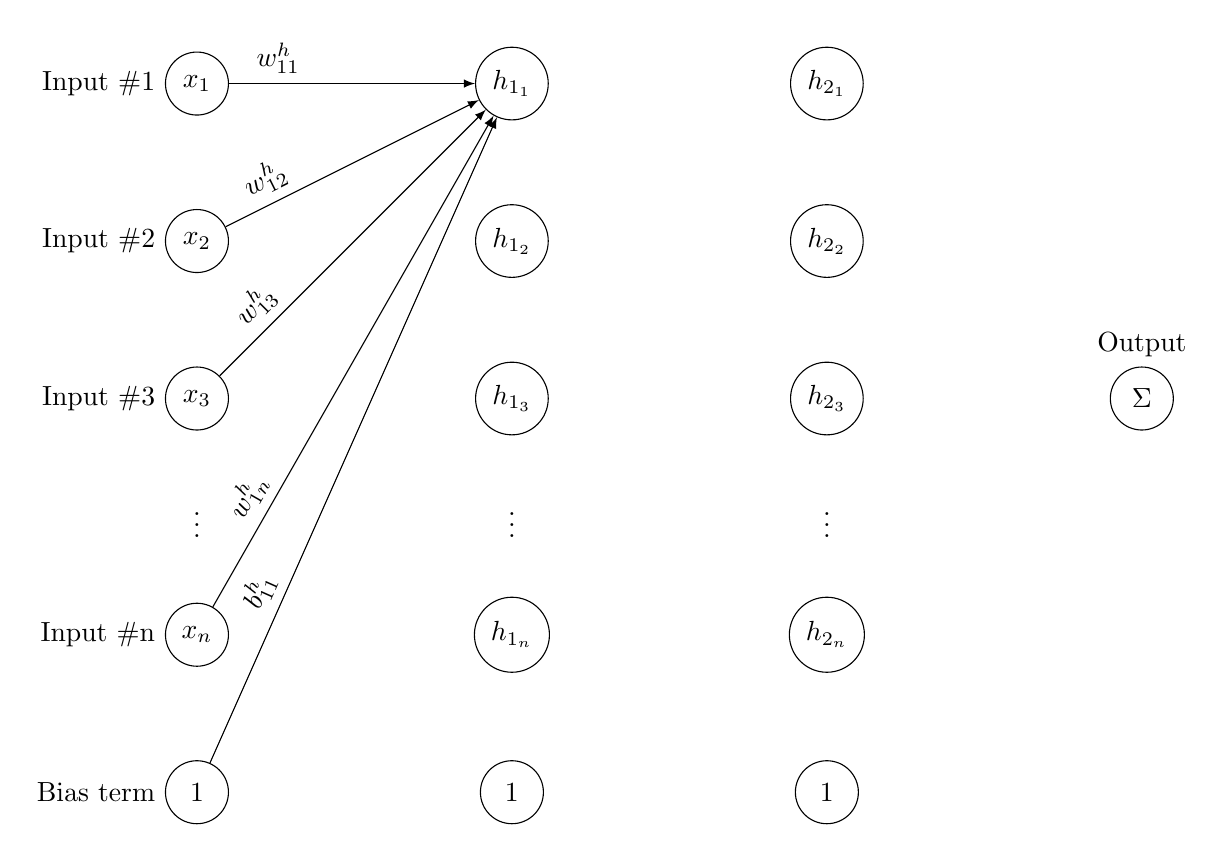
\begin{tikzpicture}
	[   cnode/.style={draw=black,draw=black,fill=#1,minimum width=8mm,circle},
	]
	\tikzset{normal arrow/.style={draw,-latex}}
	\node[cnode=white,label=90:Output] (s) at (12,-6) {$\Sigma$};
	\node at (0,-7.5) {$\vdots$};
	
	\node[cnode=white,label=180:Bias term] (x-5) at (0,-11) {1};
	
	\node at (4,-7.5) {$\vdots$};
	
	\node at (8,-7.5) {$\vdots$};
	
	\node[cnode=white,label=180:] (p-5) at (4,-11) {$1$};
	
	\node[cnode=white,label=180:] (z-5) at (8,-11) {$1$};
	
	
	\foreach \x in {1,...,4}
	{
		\pgfmathparse{\x<4 ? \x : "n"}	   
		\ifnum \x = 4
		\node[cnode=white,label=180:Input \#n] (x-\x) at (0,{-2*\x-div(\x,4)}) {$x_{n}$};
		\node[cnode=white,label=90:] (p-\x) at (4,{-2*\x-div(\x,4)}) {$h_{1_{n}}$};
		
		\node[cnode=white,label=90:] (z-\x) at (8,{-2*\x-div(\x,4)}) {$h_{2_{n}}$};
		
		\else
		
		\node[cnode=white,label=180:Input \#\pgfmathresult] (x-\x) at (0,{-2*\x-div(\x,4)}) {$x_{\x}$};
		\node[cnode=white,label=90:] (p-\x) at (4,{-2*\x-div(\x,4)}) {$h_{1_{\x}}$};
		
		\node[cnode=white,label=90:] (z-\x) at (8,{-2*\x-div(\x,4)}) {$h_{2_{\x}}$};
		
		\fi
	}
	
	
	\foreach \x in {1,...,5}
	{   
		\foreach \y in {1,...,1}
		{   
			\pgfmathparse{\x<4 ? \x : "n"}
			\ifnum \x=1
			\ifnum \y=4
			\path[normal arrow] (x-\x) -- (p-\y) node[above,sloped,pos=0.15] {};
			
			\else
			\path[normal arrow] (x-\x) -- (p-\y) node[above,sloped,pos=0.2] {$w^h_{11}$};
			\fi
			\else
			\ifnum \x=5
			\path[normal arrow] (x-\x) -- (p-\y)node[above,sloped,pos=0.25] {$b^h_{11}$}; 	
			\else
			\path[normal arrow] (x-\x) -- (p-\y)node[above,sloped,pos=0.2] {$w^h_{1\pgfmathresult}$}; 	
			\fi
			\fi
			
			
			
			
			
			
			%\draw (x-\x) -- (p-\y) node[above,sloped,pos=0.3] {$\omega_{\x\y}$};
		}
		
		
	}
	\end{tikzpicture}
	
\end{center}